\pdfobjcompresslevel=0\relax
\pdfminorversion=5\relax
\documentclass[a4paper,11pt]{article}

% ---------------------------------------------------------------------
% Language and page layout
% ---------------------------------------------------------------------
\usepackage[utf8]{inputenc}
\usepackage[T5]{fontenc}
\usepackage[english]{babel}

\usepackage{geometry}
\geometry{
    a4paper,
    left=19mm,
    right=19mm,
    top=22mm,
    bottom=22mm
}
\usepackage{setspace}
\usepackage{indentfirst}

% ---------------------------------------------------------------------
% Core mathematical and tabular packages
% ---------------------------------------------------------------------
\usepackage{float}
\usepackage{array}
\usepackage{tabularx}
\newcolumntype{L}[1]{>{\raggedright\arraybackslash}p{#1}}
\usepackage{booktabs}
\usepackage{multirow}
\usepackage{graphicx}
\usepackage{caption}
\usepackage{subcaption}
\usepackage{amsmath,amssymb}
\usepackage[table,xcdraw,dvipsnames]{xcolor}
\usepackage{tikz}
\usetikzlibrary{arrows,backgrounds,positioning,shapes.geometric}
\usepackage{enumitem}
% ---------------------------------------------------------------------
% Spacing adjustments for conference progress report format (LaTeX2e hook compliant)
% ---------------------------------------------------------------------
\makeatletter
\renewcommand\section{\@startsection{section}{1}{\z@}%
                                   {-7pt \@plus -1pt \@minus -1pt}%
                                   {3pt \@plus 1pt \@minus 1pt}%
                                   {\normalfont\large\bfseries}}
\renewcommand\subsection{\@startsection{subsection}{2}{\z@}%
                                     {-5pt \@plus -1pt \@minus -1pt}%
                                     {2pt \@plus 1pt \@minus 1pt}%
                                     {\normalfont\normalsize\bfseries}}
\makeatother
\setlength{\parskip}{1.5pt plus 0.5pt minus 0.5pt}
\setlength{\parindent}{12pt}
\setlength{\emergencystretch}{3em}

% ---------------------------------------------------------------------
% Hyperlinks
% ---------------------------------------------------------------------
\usepackage[unicode,breaklinks,plainpages=false,pdfpagelabels]{hyperref}
\hypersetup{
    urlcolor=black,
    linkcolor=black,
    citecolor=black,
    colorlinks=true
}

% ---------------------------------------------------------------------
% Bibliography
% ---------------------------------------------------------------------
\usepackage[numbers]{natbib}
\bibliographystyle{plainnat}

% ---------------------------------------------------------------------
% Header / footer
% ---------------------------------------------------------------------
\usepackage{fancyhdr}
\setlength{\headheight}{36pt}
\pagestyle{fancy}

\fancyhead{}
\fancyhead[L]{
 \begin{tabular}{rl}
    \begin{picture}(25,15)(0,0)
        \put(0,-8){\includegraphics[width=8mm]{images/hcmut.png}}
    \end{picture}
    &
    \begin{tabular}{l}
        \textbf{\ttfamily VIETNAM NATIONAL UNIVERSITY HO CHI MINH CITY}\\
        \textbf{\ttfamily HO CHI MINH CITY UNIVERSITY OF TECHNOLOGY}
    \end{tabular}
 \end{tabular}
}
\fancyhead[R]{}

\fancyfoot{}
\fancyfoot[L]{%
    \scriptsize\ttfamily
    CO5151 · Advanced Agentic Artificial Intelligence · D2 Interim Report
}
\fancyfoot[R]{%
    \scriptsize\ttfamily
    Page \thepage
}

\renewcommand{\headrulewidth}{0.3pt}
\renewcommand{\footrulewidth}{0.3pt}

\captionsetup[figure]{labelfont={small,bf},textfont={small},aboveskip=4pt,belowskip=2pt}
\captionsetup[table]{labelfont={small,bf},textfont={small},aboveskip=4pt,belowskip=2pt}

\setlength{\floatsep}{6pt plus 2pt minus 2pt}
\setlength{\textfloatsep}{6pt plus 2pt minus 2pt}
\setlength{\intextsep}{6pt plus 2pt minus 2pt}

\newcommand{\hdr}[1]{\vspace{2pt}\noindent\textbf{#1}}


\newcommand{\pending}[1]{\textcolor{red}{\textbf{[PENDING: #1]}}}
\newcommand{\code}[1]{\nolinkurl{#1}}
\begin{document}
\hypersetup{pageanchor=false}
\begin{titlepage}\begin{center}
\textbf{VIETNAM NATIONAL UNIVERSITY HO CHI MINH CITY}\\
\textbf{HO CHI MINH CITY UNIVERSITY OF TECHNOLOGY}\\
\textbf{FACULTY OF COMPUTER SCIENCE AND ENGINEERING}\\[15pt]
\includegraphics[width=2.7cm]{images/hcmut.png}\\[15pt]
{\Large CO5151 -- Advanced Agentic Artificial Intelligence}\\[12pt]
{\Huge\bfseries D2 Interim Report}\\[12pt]
{\Large LuatCheck: A Local Vietnamese Legal Assistant}\\[12pt]
Application Track -- Group 8\\[15pt]
\pending{Draft: judge validation and team confirmations remain outstanding.}\\[15pt]
\begin{tabular}{ll}
Instructor & TS. Lê Xuân Bách\\
Members & Lê Trí Quyền (2470740)\\
& Võ Phạm Tuấn Dũng (2570015)\\
& Nguyễn Hoàng Phong (2570477)
\end{tabular}\\[18pt]
\textbf{Repository:} \url{https://github.com/tuandung222/LuatCheck-D2}\\[8pt]
\textbf{Reported revision:} \pending{Insert the full final commit hash after freezing the source.}\\[8pt]
\textbf{Access:} \pending{Confirm the instructor can read the repository.}\\[8pt]
\textbf{Status:} At risk: native collection is complete; semantic validation and rehearsal remain outstanding.
\vfill HO CHI MINH CITY, OCTOBER 2026
\end{center}\end{titlepage}
\hypersetup{pageanchor=true}\setcounter{page}{1}

\section{Changes from the Proposal}
LuatCheck targets employees and SME HR staff who need an understandable answer linked to the provisions loaded into a local knowledge base. It covers a frozen original-2019 Vietnamese labour-law corpus, not all legal advice. Source implementation, unit checks and native model experiments are reported separately. Historical fallback aggregates are excluded from empirical conclusions.

\hdr{Application scenarios.} (1) An employee checks a probation or wage condition and inspects the cited article. (2) SME HR staff ask an employment question using a local model; the corpus scope and privacy limitations still apply. (3) A careless or malicious user pastes a contract with injected instructions or requests evasion of a legal duty; the system should enforce its tool boundary and ask for clarification or refuse as appropriate. These are intended scenarios, not completed user-study evidence.

\begin{table}[H]\centering\footnotesize
\begin{tabularx}{\textwidth}{@{}L{3.1cm}L{2.0cm}X@{}}
\toprule Proposal commitment & State & Delta and remaining evidence\\\midrule
Budgeted loop and citation verification & In progress & Code implemented; direct tool calls, explicit backend errors and budgets; a real native trace is reported below.\\
Qwen3-4B/8B, Qdrant and dense retrieval & In progress (changed) & Qwen2.5-3B Q4\_K\_M runs on the Mac through Metal. Explicit BM25 + TF-IDF/RRF replaces the previously proposed D2 retrieval stack. No neural result is claimed.\\
Embedding support and optional L2 & In progress (changed) & Lexical and exact-quantity checks are proxies, not semantic guarantees. Semantic judging and threshold calibration remain unvalidated. The previous heuristic NLI substitute has been removed.\\
Ten native tasks at D2 & In progress (scoring) & Sixty native trials on ten source-checked local tasks are collected, including twelve model-output errors. Semantic scoring remains pending; no public VLQA provenance is claimed.\\
HR walkthrough in W5 & Not started & The group reported on 22 October that the walkthrough has not taken place. No user-study result is claimed. \pending{Confirm the rescheduled date and owner.}\\
Initial attack results & Dropped (D2 claim) & Historical input-filter diagnostics do not establish retrieved-shard or physical egress safety. Final attack evaluation remains planned.\\
\bottomrule\end{tabularx}
\caption{Commitment comparison. Source implementation does not establish measured model performance.}
\end{table}
The group reported on 22 October that no pitch feedback has yet been received; no feedback-driven changes are claimed.
The model/retrieval changes limit resource use and make the actual statistical method explicit. The revised verification claim is limited to checks implemented in code. Team-confirmed final statuses must use done / in progress / not started / dropped.

\section{Implemented Architecture (R1)}
The application currently uses one agent. Its ReAct-style loop~\citep{yao2023react} calls a Python tool registry directly; the separate MCP server is not a transport used by the main loop. No multi-agent coordination is claimed.
This pattern permits additional source lookup and bounded repair after a failed check. A single controller keeps tool permissions and budgets inspectable on one local machine. Its benefit over the simpler OFF configuration remains an empirical question.
\begin{figure}[H]\centering
\begin{tikzpicture}[node distance=0.28cm,
block/.style={draw,rounded corners,align=center,text width=12.5cm,minimum height=0.62cm,font=\small},
arrow/.style={->,>=stealth}]
\node[block] (input) {Question / optional document: input checks and untrusted-data delimiters};
\node[block,below=of input] (llm) {Native Ollama / llama.cpp client; bounded action loop\\Backend/format error becomes an explicit error, never a substitute answer};
\node[block,below=of llm] (tools) {Direct registry: search and article lookup\\BM25 + TF-IDF/RRF; observations retained in the session ledger};
\node[block,below=of tools] (verify) {OFF: verification removed \quad ON: ID, provenance, lexical and quantity checks};
\node[block,below=of verify] (end) {Pass: answer and optional verified memory write\\Failure: bounded repair or refusal; missing details: clarify; execution failure: error};
\draw[arrow] (input)--(llm);\draw[arrow] (llm)--(tools);
\draw[arrow] (tools)--(verify);\draw[arrow] (verify)--(end);
\end{tikzpicture}
\caption{Implemented control path. A separate trusted UI can approve a local-outbox proposal. External email delivery is not implemented. Whole-system quality validation remains pending.}
\end{figure}
The frozen main limits are five tool calls, two repairs, eight loop steps, 180 seconds per task and 768 output tokens per generation. The native timeout is 60 seconds, bounded by the remaining task deadline. These are configured limits, not measured latency. Backend errors are distinct from safety refusals. A budget stop may appear as a refusal in the controller ledger; it is not evidence of an appropriate safety decision.

\hdr{Observed native task trace.}
For \code{BLL19-01-PROBATION}, seed 42, ON: the model issued \code{search_law} for the probation-period question; it then called \code{get_article(Dieu_25)} because search returned a truncated snippet. Reading the complete article exposed clause 2. The next native action answered \emph{60 days} and cited its actual text. The configured L1 checks passed, with two tool calls, zero repairs and three native generations: 7,456 input and 448 output tokens, 16.627 seconds end-to-end. This establishes this observed task, not general legal accuracy. The full requests, responses and observations are retained in \code{evaluation/runs/bll2019-main-v2/runs.jsonl}; the runtime source snapshot is stored beside it.

\section{Tools and Permissions (R2)}
\begin{table}[H]\centering\footnotesize
\begin{tabularx}{\textwidth}{@{}L{2.6cm}L{2.5cm}X@{}}
\toprule Interface & State / permission & Enforced boundary\\\midrule
\code{search_law} & Implemented; read-only & Reads the configured article corpus.\\
\code{get_article} & Implemented; read-only & ID lookup returns local source text.\\
Agent memory write & Implemented; reversible write & SQLite write follows the agent verification gate; that gate is not independent legal validation.\\
MCP \code{save_case} & Write blocked & Model caller cannot self-attest verification; no SQLite write through this tool.\\
\code{send_summary} & Proposal only & Model-facing tool cannot approve or execute.\\
Trusted UI outbox & Implemented; reversible local write & Conservatively gated: host approval/token bound to payload. Caller boolean alone is insufficient. Queue receipt is not delivery.\\
External sender; code execution & Not implemented & No email/webhook transport or arbitrary-code tool is claimed.\\
\bottomrule\end{tabularx}
\caption{Tool state and permissions. Runtime and MCP-transport demo evidence must match the interfaces actually presented.}
\end{table}
Outbox failures must not produce a delivery receipt. Identical payload/key pairs are deduplicated locally. The demo targets a single user/process; multi-user isolation and cross-process outbox guarantees are not certified.
A local stdio MCP integration check confirmed tool discovery, search, article lookup, blocked unverified writes and proposal-only summaries. The script and result are in \code{docs/reviews/native-integrity-revision-2026-10-22}. This is tool-contract evidence, not a native model task. \pending{Attach the actual application demo evidence.}

\section{Memory and Knowledge Sources (R3)}
\hdr{Short-term state.} The ledger stores the question, issued searches, retrieved IDs/text, budgets, action/verification events and native-call telemetry. It supports task inspection, not another autonomous agent.

\hdr{Episodic memory.} The agent writes answers following its configured verification gate and native-call evidence. Query, answer and citation strings undergo supported-pattern filtering. Reuse requires matching index version, native-origin metadata and similarity threshold 0.85. Legacy records without native-origin metadata are skipped; records are retained, not silently relabelled. The similarity combines TF-IDF cosine and Jaccard. Cached answers are rechecked in the selected verification mode. D2 experiments disable memory reads/writes. Pattern filtering is incomplete data minimisation, not proof of legal compliance or removal of all personal data. Native-origin metadata assumes trusted code/storage; it is not a signed backend attestation.

\hdr{Knowledge corpus.} The current retrieval corpus contains all \textbf{220 numbered articles} of the original Labour Code 45/2019/QH14 in the official Gazette dated 26 December 2019~\citep{bll2019gazette}. It is not a consolidated representation of current 2026 law. The 94-page text PDF, SHA-256 manifest, extraction script and page-level text are preserved in \code{docs/materials/benchmark-sources}. Each retrieval record has its source URL, source-PDF hash and page numbers. Extraction removes running Gazette headers, normalises Unicode/whitespace and segments article headings; it does not rewrite legal provisions. Automated checks establish unique coverage of articles 1--220 and exact containment of the selected reference excerpts.

BM25 indexes titles/content; TF-IDF uses word n-grams 1--3. RRF uses $k=60$. Each search component considers twice the requested result count; the final count is capped at five. No neural embedding is silently substituted. The separate SOP demonstration is outside the frozen experiment. Source checking and task curation were assisted by OpenAI Codex; \pending{a legal expert has not yet certified the corpus extraction, task conditions or gold answers.}

\clearpage
\section{Evaluation Set and Initial Results (R5)}
\hdr{Benchmark provenance and selection.}
\code{evaluation/benchmarks/bll2019_v1/tasks.json} contains ten purposively selected, source-grounded local tasks: seven single-provision questions, two multi-article synthesis questions and one foreign-jurisdiction refusal. The nine answerable tasks have frozen reference answers and exact source excerpts with Gazette page numbers. The original drafts were revised before main outputs: an inconsistent contract-duration scenario was removed, disciplinary dismissal was distinguished from unlawful unilateral termination, notice-period exceptions were stated, and the explicit contract-guarantee deposit question was corrected to be answerable under Article 17. No task or gold is changed to fit model output.

These are \textbf{local curated tasks, not a verified public VLQA split}. The legacy VLQA record mapping could not be established; ALQAC file access was restricted and was not bypassed. The source-review manifest names the AI reviewer and marks expert review pending. This small development set does not establish broad or held-out legal performance. The proposal's final targets of twenty end-to-end tasks and 200 held-out retrieval pairs remain separate work.

\hdr{Native configurations and controls.}
OFF and L1 ON use the same Qwen2.5:3B Q4\_K\_M model, prompt, corpus, budgets and explicit BM25/TF-IDF retrieval. OFF removes verification; ON checks citation existence, retrieved provenance, verbatim-quote containment, lexical overlap and quantities, then permits bounded repair. Optional NLI requires a real native model and is excluded from this comparison. There are no response substitutes, injected stand-in components or answer-cache hits. Episodic memory is disabled by a real configuration flag, rather than replacing methods.

The first environment is the user's Apple M4, 10 CPU cores and 16 GiB unified memory. Ollama 0.34.4 reports Metal placement, 8,192 context tokens and model allocation in GPU memory. Runs are sequential. Seeds 42, 123 and 2026 are passed to the native API; OFF/ON order alternates by task. Three seeds repeat ten tasks, not thirty independent legal questions. Native prefix caching is backend behaviour; response-cache reuse is disabled. Some software checks and report compilations ran on the same Mac during collection; no second model inference workload was run concurrently. Timings are observations of this desktop environment, not isolated throughput or causal speedup measurements.

\hdr{Measured metrics and semantic judging.}
Retrieval recall counts the fraction of gold IDs recovered; hit and MRR remain distinct. Trajectory Recall/Hit@5 use the first five unique IDs accumulated during the tool trace; MRR uses the first relevant ID in the complete ordered unique trajectory. Neither is a separate held-out retrieval test. Citation-ID precision/recall use the reference ID set and are aggregated only over answerable trials. Empty-gold foreign-scope rows have no applicable source-ID recall; their raw legacy convention is excluded. These do not establish whether a cited provision entails a claim. Gold ID sets may also omit a valid alternative source; semantic review must inspect the actual text rather than equate ID mismatch with a wrong answer. Separating answer correctness from citation support follows the evaluation distinction in ALCE~\citep{gao2023alce}.

Latency includes the agent loop; tokens come from native usage fields, including additional repairs. Missing usage stays unknown. Model service-hours sum backend request durations on the Metal-backed model; they are \emph{not} a hardware GPU-active measurement. A local API fee is not a claim of free compute.

Task correctness, completeness, claim support and the appropriateness of refusal/clarification require semantic review. The prepared judge protocol supplies question, frozen reference/rubric, source articles and a blinded candidate answer; it excludes OFF/ON and L1 acceptance. Judge bias and agreement with human ratings must be checked rather than assumed~\citep{zheng2023judge}. \pending{Record the actual independent judge, settings, responses, semantic metrics and reliability on a human-labelled sample.} Regex/L1 acceptance and reference token F1 cannot fill that slot. Source-ID metrics, reference exact match/token F1 and lexical unsupported rate are reported only in their stated roles.

\input{native_results.tex}
The complete main batch records 264 native calls and complete token usage for all 60 trials. OFF returned 18 answers and had 5 model-output errors; ON returned 14 answers and had 7 such errors. These are action/status counts, not correctness labels. The observed source-ID metrics do not establish an improvement from L1, and no semantic superiority is claimed. An earlier ten-trial attempt was interrupted and remains excluded from these aggregates.


\hdr{Pilot findings and limitations.}
The first pilot retained eight native trials. The controller sometimes asked users for statutory information hidden beyond a 300-character snippet; it also produced a legally wrong synthesis that passed L1. Search responses were changed to expose truncation explicitly and the prompt now requires reading the full article instead of treating a snippet's omission as missing user facts. A second four-trial interface pilot retained all outputs, including an unnecessary clarification. Neither pilot is merged into main results or presented as held-out validation.

A concrete first-pilot failure conflated the notice period with service time used for severance in Article 46. This illustrates why lexical acceptance cannot be called legal correctness. Main failures and raw native responses, including parse errors, truncation and deadlines, remain in the result artifact. There is no statistically established superiority claim from this small set. The saved backend log also records context shifting in some calls at the configured 8,192-token limit. Full request text is retained, but that does not establish that all earlier evidence remained in the model's active context. Reducing duplicate observation fields or increasing context requires a separately versioned rerun, rather than revising this frozen batch.

\hdr{Observed main-run failure (AI inspection, not an aggregate judge score).}
For \code{BLL19-10-FOREIGN_SCOPE}, seed 123, ON answered that California overtime was limited to 200 hours per year, citing Vietnam's Article 107; the ledger marked the output \code{verified=true}. The configured corpus contains only the original Vietnamese statute and supplies no California authority. This is a concrete jurisdiction/support failure that the implemented L1 checks did not reject. Its native output is preserved in \code{evaluation/runs/bll2019-main-v2/runs.jsonl}. Independent semantic scoring remains pending; this qualitative case does not supply a benchmark accuracy estimate.

\hdr{Reproduction.}
Native collection and recomputation instructions, frozen task/corpus hashes and environment metadata accompany the run directory. \pending{Freeze the final reported source commit and confirm instructor access.} Missing semantic/human evidence remains red; operational metrics must be recomputed from the actual native artifacts.
\clearpage
\section{Threat Model (R6)}
An attacker can craft questions/documents and, in a separate future poisoning test, a lower-trust retrieved item. The attacker cannot modify trusted code, the approved reference corpus or trusted UI approval state under the current assumptions.
\begin{table}[H]\centering\footnotesize
\begin{tabularx}{\textwidth}{@{}L{2.3cm}L{2.4cm}X@{}}
\toprule Entry / asset & Attacker capability & Boundary and remaining risk\\\midrule
Question / answer integrity & Arbitrary instructions & Pattern checks, delimiters, fixed dispatch; paraphrase bypasses remain possible.\\
Pasted document / case data & Embedded directives & Untrusted delimiters and read-only lookup; assess bypasses and benign false positives later.\\
Retrieval/tool text / evidence & Poison returned text & ID/provenance and support review; input-filter tests do not establish retrieved-shard resistance.\\
Memory / privacy & Request prior cases & Versioned/rechecked memory, no dump tool; user-level isolation remains a deployment risk.\\
Audit / personal data & Supply sensitive strings & Recursive supported-pattern filtering; retention and remaining data categories need review.\\
Outbox / unauthorised write & Request action or forge flag & Proposal-only tool; host approval/token bound to payload. Local queue only, no network sender.\\
Resources / availability & Long or invalid action loops & Tool/repair/step/time/token bounds; errors are not counted as successful defense.\\
\bottomrule\end{tabularx}
\caption{System-specific threat model. Mitigations are implementation boundaries, not measured attack-effectiveness guarantees.}
\end{table}
D2 does not require injection experiments. Final tests will place payloads at their actual entry points, check attacker objectives using tool/outbox receipts and measure legitimate correctness separately. Historical 100\% defense/utility claims are excluded.

\section{Weekly Plan to the First Final Presentation}
\begin{table}[H]\centering\footnotesize
\begin{tabularx}{\textwidth}{@{}L{1.7cm}L{2.0cm}X@{}}
\toprule Week / date & Proposed owner & Deliverable / acceptance\\\midrule
Before 25 Oct & All & Complete native collection, independent judge and human audit; confirm gold, report, slides and backup video.\\
W45, 2--8 Nov & Quyền / Phong & Document HR walkthrough status/findings, corpus provenance and scenarios.\\
W46, 9--15 Nov & Dũng / Quyền & Expand approved tasks; independently audit verifier and answer failures.\\
W47, 16--22 Nov & Phong / Dũng & Real entry-point attack tests and permission/fault checks; inspect committed effects.\\
W48, 23--29 Nov & All & Frozen-artifact reproduction, demo hardening, final report. Optional NLI/reranking only after core evidence.\\
W49, 30 Nov--2 Dec & All & Tagged release, final checks and Round 1 presentation on 2 December.\\
\bottomrule\end{tabularx}
\caption{Proposed plan. \pending{Team to confirm owners, walkthrough dates and commitments.}}
\end{table}
The riskiest assumption is that the native 3B controller answers correctly within budget. Real pilots exposed source-reading and semantic errors. If the pilot is slow, keep ten approved tasks and two configurations; cut expansion, optional NLI/reranking and external delivery. Preserve the real loop, trace, bounded tools, human-scored outputs and reproducibility. If native results remain unavailable, state the missing requirement rather than substitute simulated numbers.
\textbf{Self-assessment: at risk}, pending validated semantic judging, team confirmations and demo rehearsal.

\clearpage
\section{Member Contributions and AI-Use Statement}
\begin{table}[H]\centering\footnotesize
\begin{tabularx}{\textwidth}{@{}L{3.2cm}X L{3.0cm}@{}}
\toprule Member & Earlier draft responsibilities & Attribution evidence\\\midrule
Lê Trí Quyền & Retrieval and corpus & \textcolor{red}{Evidence pending}\\
Võ Phạm Tuấn Dũng & Agent, verifier and evaluation & \textcolor{red}{Evidence pending}\\
Nguyễn Hoàng Phong & Tools, security and UI & \textcolor{red}{Evidence pending}\\
\bottomrule\end{tabularx}
\caption{The group has not yet supplied confirmed contribution/verification evidence. Earlier responsibility labels are not completed-work claims.}
\end{table}
The earlier draft named Claude and GitHub Copilot for scaffolding and formatting. This revision also used OpenAI Codex for source review, native-only runtime changes, test maintenance, report restructuring and experiment planning.
\pending{Confirm the full AI tool list and actual uses, including other assistants if used. Model authorship cannot be inferred from code quality.}
Native measurements are collected on the Mac under the frozen protocol. The earlier 509-test suite contained substitutions and was retired following the user's stricter requirement. Its count is not evidence for this revision. The replacement suite exercises real source data, retrieval, storage, MCP transport and native inference; the post-collection run passed all 11 tests in 43.31 seconds. These test results do not replace benchmark quality measurements.
The group reported on 22 October that member-specific contribution/verification evidence is not yet available. \pending{Supply actual member checks and supporting commits/artifacts before submission.} AI-assisted work is not attributed to a member or a human expert without confirmation.

\bibliography{refs}
\end{document}
